\section{模型实验}
\label{sec:model}

\subsection{实验框架的实现}

\subsection{随机森林}
    展示结果即可:sfcc/gsd/server/sprint.bash
    其中没注释的命令跑一下,画feature importance
	这个图位置总不对。。。
	\begin{figure}[!htb]
	    \centering
	    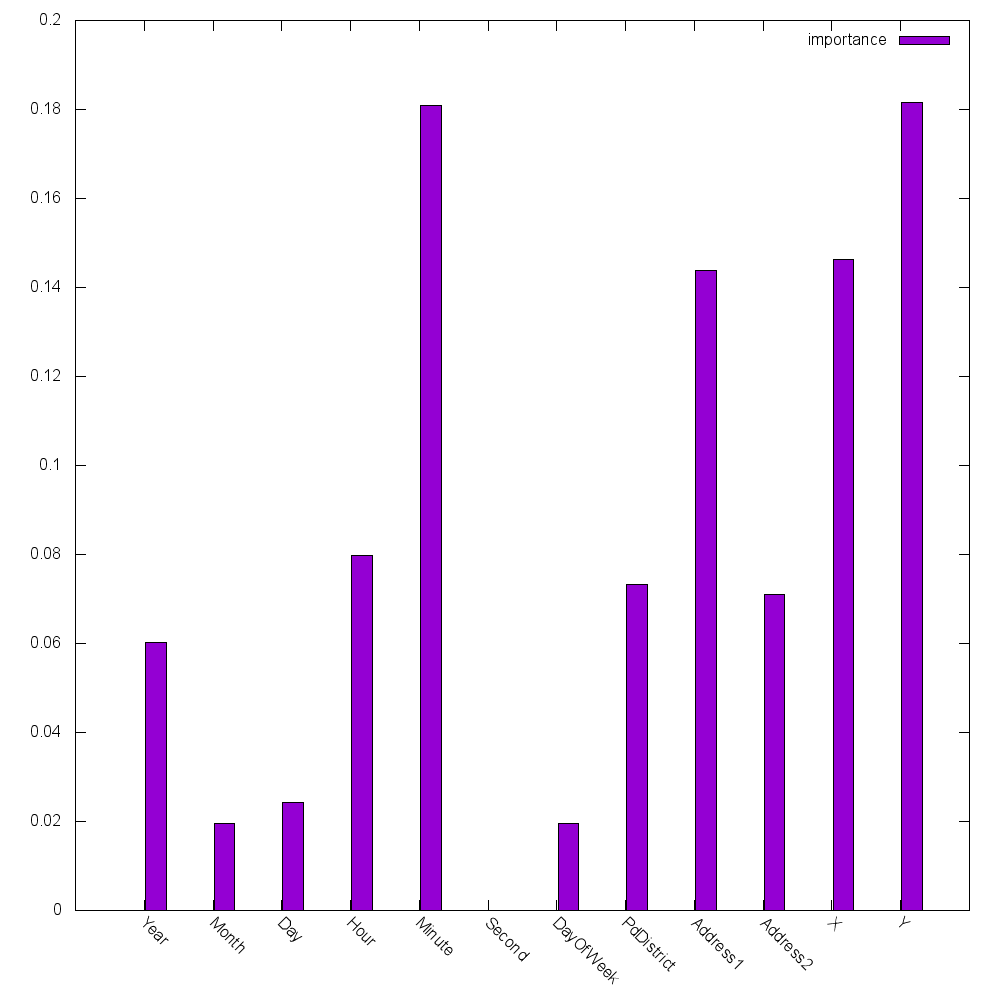
\includegraphics[width=1.0\linewidth]{fig/importance}
	    \caption{特征重要性}
	    \label{importance}
	\end{figure}

\subsection{Xgboost}
我们最终提交的结果是Xgboost跑出的结果,Xgboost在本次竞赛中相比其它我们使用的模型效果要出色很多。
下表是我们各次提交的结果:

\begin{tabular}{|p{0.4cm}|p{0.4cm}|p{0.4cm}|p{0.4cm}|p{0.4cm}|p{0.4cm}|p{0.4cm}|p{1.2cm}|p{1.2cm}|}
\hline
提交编号 & 使用特征编号 & 迭代轮数 & 决策树最深宽度 & 学习率 & 每棵树的列采样率 & 提交结果保留几位小数 & 本地检验结果 & 提交结果 \\
\hline
1 & 0 & 60 & 8 & 0.3 & 1 & 3 & 2.22376 & 2.31334 \\
\hline
2 & 0 & 100 & 8 & 0.1 & 1 & 3 & 2.259029 & 2.29657 \\
\hline
3 & 0 & 100 & 10 & 0.1 & 1 & 3 & 2.235178 & 2.29852 \\
\hline
4 & 0 & 100 & 6 & 0.1 & 1 & 3 & 2.289943 & 2.31782 \\
\hline
5 & 0 & 200 & 6 & 0.1 & 1 & 3 & 2.263382 & 2.31364 \\
\hline
6 & 4 & 200 & 6 & 0.1 & 1 & 3 & 2.208462 & 2.64618 \\
\hline
7 & 3 & 200 & 6 & 0.1 & 1 & 3 & 2.24326 & 2.43281 \\
\hline
8 & 5 & 200 & 6 & 0.1 & 1 & 3 & 2.229024 & 2.30504 \\
\hline
9 & 3 & 200 & 8 & 0.1 & 1 & 3 & 2.223634 & 2.46337 \\
\hline
10 & 5 & 200 & 8 & 0.1 & 1 & 3 & 2.21475 & 2.33183 \\
\hline
11 & 3 & 100 & 3 & 0.1 & 1 & 3 & 2.313002 & 2.40017 \\
\hline
12 & 0 & 100 & 3 & 0.1 & 0.8 & 3 &  & 2.2875 \\
\hline
13 & 0 & 100 & 8 & 0.1 & 0.8 & 3 & 2.2503 & 2.28598 \\
\hline
14 & 0 & 100 & 8 & 0.1 & 0.8 & 5 & 2.2503 & 2.25392 \\
\hline
15 & 3 & 200 & 8 & 0.1 & 0.6 & 5 &  & 2.26982 \\
\hline
16 & 0 & 200 & 8 & 0.1 & 0.8 & 5 &  & 2.23887 \\
\hline
\end{tabular}

由于随机选取参数的Xgboost模型就取得了比之前随机森林模型的结果要好很多的结果,使得我们对Xgboost很有信息,因此花了很多时间来调参数。
1~5次提交是我们刚刚开始尝试Xgboost模型,随意选取了几组参数进行测试,我们主要调整的几组参数为迭代轮数和决策树最大高度。可以发现Xgboost
的模型抗过拟合效果良好,通常只要增加迭代轮数,无论再小都会有所提升。另外,过高或者过低的决策树高度都是不合适的,低一点的决策树高度会导致
决策表达能力不足,高一点的决策树深度会导致过拟合,并且训练时间会长不少。

进行了简单的尝试之后,我们尝试了之前在随机森林模型下取得更好结果的特征三和特征四进行测试,得到了编号6和编号7的数据。令我们大跌眼镜的是,
这两个特征在测试集上取得了更好的结果,但是提交之后的结果变差了很多,这让我们开始怀疑特征三和特征四由于蕴含了训练集的结果,导致了这个情况
的出现,因为这两个特征都直接加入了对测试集标签的统计信息。但由于不能确定是否是参数导致的问题,我们又跑出了编号9的结果,没有明显改善。

为了搞清楚是否是特征三和特征四的问题,我们换了间接使用结果信息的特征五来进行训练和预测,提交得到了编号8的结果,与之前获得的最好的结果差距不大。
因此我们希望进一步挖掘特征五的潜力,看在参数的调整下是否能获得更进一步的提升。于是我们提交了编号10的结果,出乎意料的结果变差了,而编号8和编号10的
区别只有最高决策树高度这一参数。因此我们怀疑是对于此类引入训练集结果信息的特征,模型表达能力越强越容易过拟合。因此我们决定接下来使用不引入结果信息
的特征零来进行训练和预测。

在这之后,我们陷入了一段瓶颈期,测试各种参数的组合得到的本地结果并没有迹象能比较有效的超过编号2的结果。于是我们决定引入新的变量以求的到提升,在
查阅文档之后,发现Xgboost提供了列采样率这一参数,就是说对于每轮建立的新的决策树,并不把特征的所有列作为决策树需要分类的数据,而是随机的选取其中的
一部分作为决策树需要分类的数据。这个参数能使得各轮训练得到的决策树区别变大,由于我们的特征维数并不高,容易导致决策树的同质化,因此我们认为这个参数
会带来较大的提升。调整了这个参数之后,我们得到了编号12的结果,终于得到了优于编号2的结果的结果。

编号12的参数的决策树最高高度较低,主要是因为我们发现了SKlearn的Gradient Boost模型的默认参数中决策树最高高度为3,因此做这个尝试,但是根据本地训练
过程中的数据,我们认为对于这个问题该参数还是大一点比较好,于是我们将该参数调高之后得到了编号13的结果,有所提升,但是不甚明显,这与我们本地数据出入很大。
这也是我们之前的结果出现的一个普遍问题,本地测试的结果与提交结果差别较大,解决这个问题得到编号14的结果也是灵光乍现。之前由于提交文件过大,我们的结果文件
只保留三位小数来减小提交文件的大小。但是对于本问题,预测的准确率不超过30\%,因此预测误分类的几率还是很大的,而对于这个比赛的评分方式,假如误分类,并对于
正确分类给出的概率较低,即使是小数点后四位的差别也会导致最终评分增加很多。想到这点之后我们将结果文件保留了五位小数,提交后得到编号14的结果,基本消除了本地
测试和提交结果的区别,不再过拟合测试集数据。

之后我们由于距离提交时间非常接近,而且进行一次模型的训练要花很久的时间,所以最后两次结果没有进行分折测试,直接提交了结果。其中编号16的结果使用的参数
只对于编号14的参数改动了迭代轮数,利用了Xgboost模型不宜过拟合的特性,取得了我们最终的成绩。

\subsection{K最近邻}
    使用原来的数据和未规格化的数据分别做3000近邻的分类。
    命令 sfcc/gsd/server/knn.bash
	
	fold 1: logloss=2.65553851001; accuracy=0.206650533808

	fold 2: logloss=2.6579303191; accuracy=0.205918696224

	fold 3: logloss=2.65923152836; accuracy=0.206496176208

	fold 4: logloss=2.65677336961; accuracy=0.206037447894

	fold 5: logloss=2.65510318698; accuracy=0.205938631859

	average: logloss=2.65691538281; accuracy=0.206208297199

\subsection{逻辑斯蒂回归}
    重新构造特征之后的实验结果。